\documentclass[tikz,border=10pt]{standalone}
\begin{document}
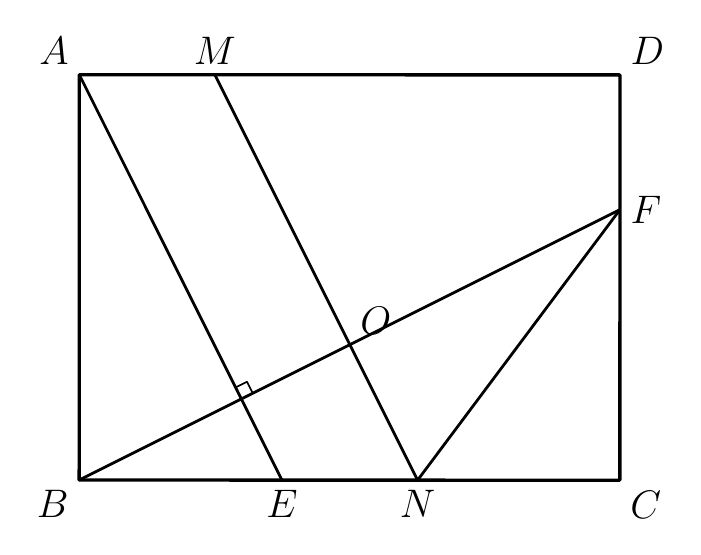
\begin{tikzpicture}[line width=1.0pt, line join=round]
% Named coordinates (scale s=0.018141, centre (257,207) px)
\coordinate (A) at (-3.43211554629554,2.575401955874486);
\coordinate (B) at (-3.433810450188731,-2.5719490923945996);
\coordinate (C) at (3.433018164033461,-2.5742101805626643);
\coordinate (D) at (3.4347130679266527,2.573140867706421);
\coordinate (M) at (-1.7095660788613105,2.574834760093357);
\coordinate (E) at (-0.8581063987016976,-2.572797212288431);
\coordinate (N) at (0.8644430687325318,-2.57336440806956);
\coordinate (F) at (3.4341495991931468,0.8619102854130962);
\coordinate (O) at (0.004274574161485828,-0.852966975772105);
% Right-angle square corners (vertex V and mark points)
\coordinate (V) at (-1.37500000000000,-1.54400000000000);
\coordinate (P1) at (-1.22900000000000,-1.47050000000000);
\coordinate (P2) at (-1.30250000000000,-1.32400000000000);
\coordinate (P3) at (-1.44850000000000,-1.39750000000000);

% Rectangle ABCD, sides at 1.2pt to match original weight
\draw[line width=1.2pt] (A) -- (D) -- (C) -- (B) -- cycle;
% Segments AE, MN, BF, FN
\draw (A) -- (E);
\draw (M) -- (N);
\draw (B) -- (F);
\draw (F) -- (N);
% Single right-angle mark at V (BF perpendicular to AE), closed square, thin stroke
\draw[line width=0.6pt] (V) -- (P1) -- (P2) -- (P3) -- cycle;

% Labels
\node[above left, font=\fontsize{14.5}{17.4}\selectfont] at (A) {$A$};
\node[above right, font=\fontsize{14.5}{17.4}\selectfont] at (D) {$D$};
\node[above, font=\fontsize{14.5}{17.4}\selectfont] at (M) {$M$};
\node[below right, font=\fontsize{14.5}{17.4}\selectfont] at (C) {$C$};
\node[below left, font=\fontsize{14.5}{17.4}\selectfont] at (B) {$B$};
\node[below, font=\fontsize{14.5}{17.4}\selectfont] at (E) {$E$};
\node[below, font=\fontsize{14.5}{17.4}\selectfont] at (N) {$N$};
\node[right, font=\fontsize{14.5}{17.4}\selectfont] at (F) {$F$};
\node[above right, font=\fontsize{14.5}{17.4}\selectfont] at (O) {$O$};
\end{tikzpicture}
\end{document}
% GEOAGENT_REPAIR_V1 c18a466396f54661 bf4342b0097ccd59a21cdcc8891f725fc4614f36aba98f24a3305b667dadc1f0